\section{Data Processing}
\label{sec:data-processing}

\subsection{Trigger}
As described in section \ref{sec:dom-daq}, the high-frequency ATWD waveform digitization in each DOM is triggered when it and its adjacent or next-to-adjacent neighbors on the same string record a voltages of at least 0.25 PE-equivalent within a $\pm$1~$\mu$s time window, which is referred to as the Hard Local Coincidence (HLC) condition. Data acquisition for DeepCore is triggered when this condition is fulfilled for at least three DOMs inside the DeepCore fiducial volume within a $\pm$2.5~$\mu$s window. If this condition is met, the waveforms for all DOMs that have observed voltages of at least 0.25~PE within a $\pm$10~$\mu$s time window centered around the trigger time are recorded. A DOM that is included in this readout but for which the HLC condition has not been met is said to fulfill the \emph{Soft Local Coincidence} (SLC) condition. The DeepCore trigger rate is less than 10~Hz and will trigger on \~70\% of $\nu_\mu$ events at 10~GeV and >90\% of $\nu_\mu$ events at 100~GeV\cite{DeepCore}.

\subsection{Online Filter}

Once the trigger condition is met, the recorded waveforms within the trigger window are converted into reconstructed pulses and are then passed into a set of \emph{online} filters (i.e. filters running on hardware at the Pole). These filters are each designed to select events that are relevant to different physics measurements that are performed within the IceCube collaboration. For the purposes of the analysis presented in this thesis, events are selected using the \emph{DeepCore filter}. This filter is designed to select events that start inside the DeepCore fiducial volume and to reject those that are consistent with muons entering the detector from the outside.
\begin{marginfigure}
    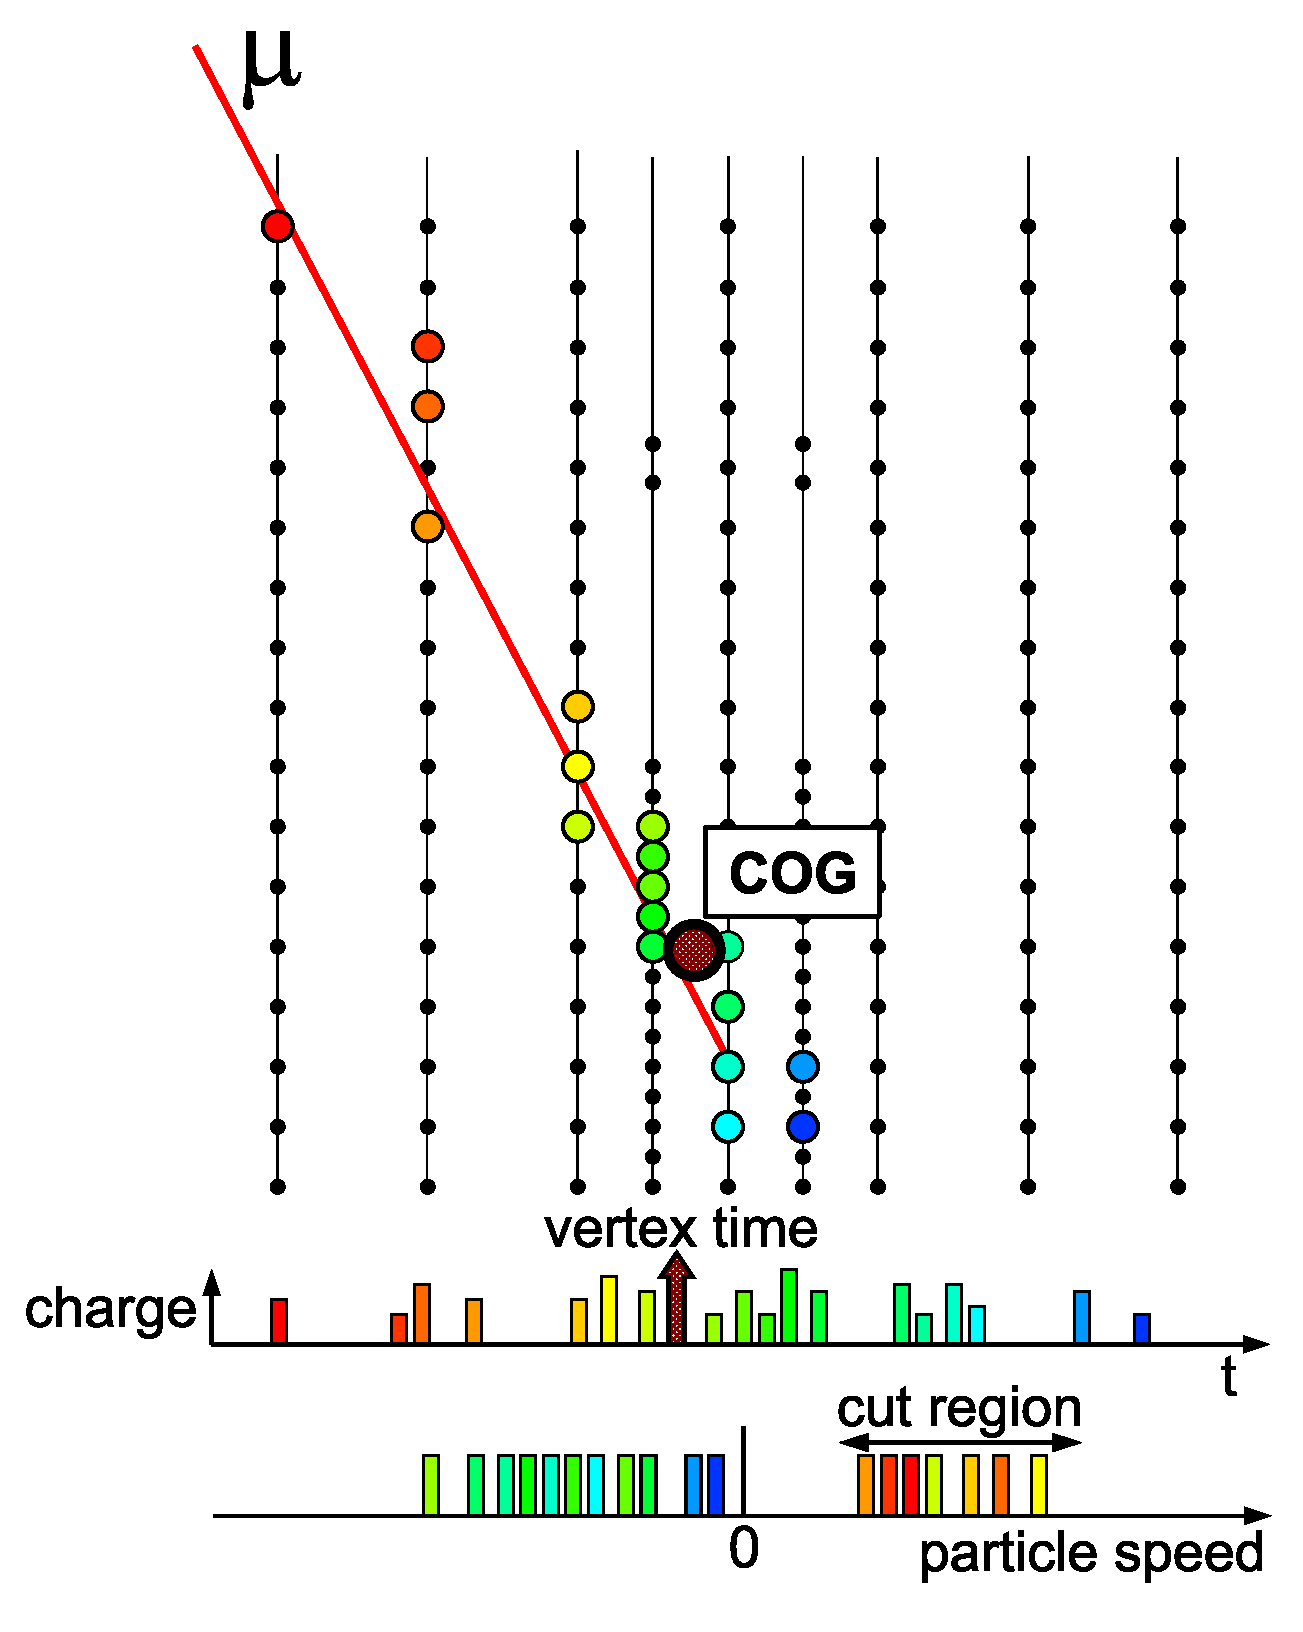
\includegraphics[width=\textwidth]{figures/icecube/eventviews/FilterDiagram.pdf}
    \caption{Example of an event that would be rejected by the online filter algorithm. DOMs that have observed light are highlighted in color depending on time from red (early hits) to blue (late hits). DOMs that have not observed any light are shown as black dots. Figure taken from \cite{DeepCore}.}
    \label{fig:online-filter-event}
\end{marginfigure}
The filter first applies a noise cleaning algorithm based on a coincidence condition between hits on different DOMs, where hits in DOMs for which the HLC condition was met are always kept. The cleaned hit series is split between those hits that fall within the DeepCore fiducial volume and those outside of it. The veto algorithm then calculates the COG in space and time of the hits inside the fiducial volume and then the velocity that a signal would have to travel from each hit occurring outside the fiducial volume to coincide with the COG. If this velocity is close to the speed of light (between $0.25\;\mathrm{ns/s}$ and $0.4\;\mathrm{ns/s}$) for at least one hit, the event is rejected because it is consistent with a muon traveling through the veto region and entering DeepCore. Figure~\ref{fig:online-filter-event} shows an example of an event that would be rejected by the online filter. Only events passing the trigger and filter condition are sent North via satellite for further \emph{offline} filtering.

\subsection{Offline Filter}

The offline filter is separated into subsequently applied \emph{levels}, referred to as L3, L4, and L5, where each level reduces the amount of background (atmospheric muons and noise) by approximately an order of magnitude while keeping most of the DeepCore starting events that are the target of the selection.

\subsubsection{Level 3}
At the lowest offline filter level, L3, cuts are applied to simple variables that remove the most easily identifiable background events while using only few computational resources. The variables aimed at cutting noise consist mostly of different DOM hit counts within hit series to which noise cleaning algorithms have been applied. The cuts aimed at removing muons consist of conditions on the number of hits in the veto region as well as conditions on the vertical position of the first HLC hit. The distribution for one of the variables used in the L3 filter is shown in figure~\ref{fig:l3-var-cleaned-full-time-length}. It is apparent from the distributions that there is a significant population of events in data with large values of the plotted variable that does not exist in simulation. These events are discarded, improving the agreement between data and simulation for events passing the L3 filter.
\begin{figure}
    \centering
    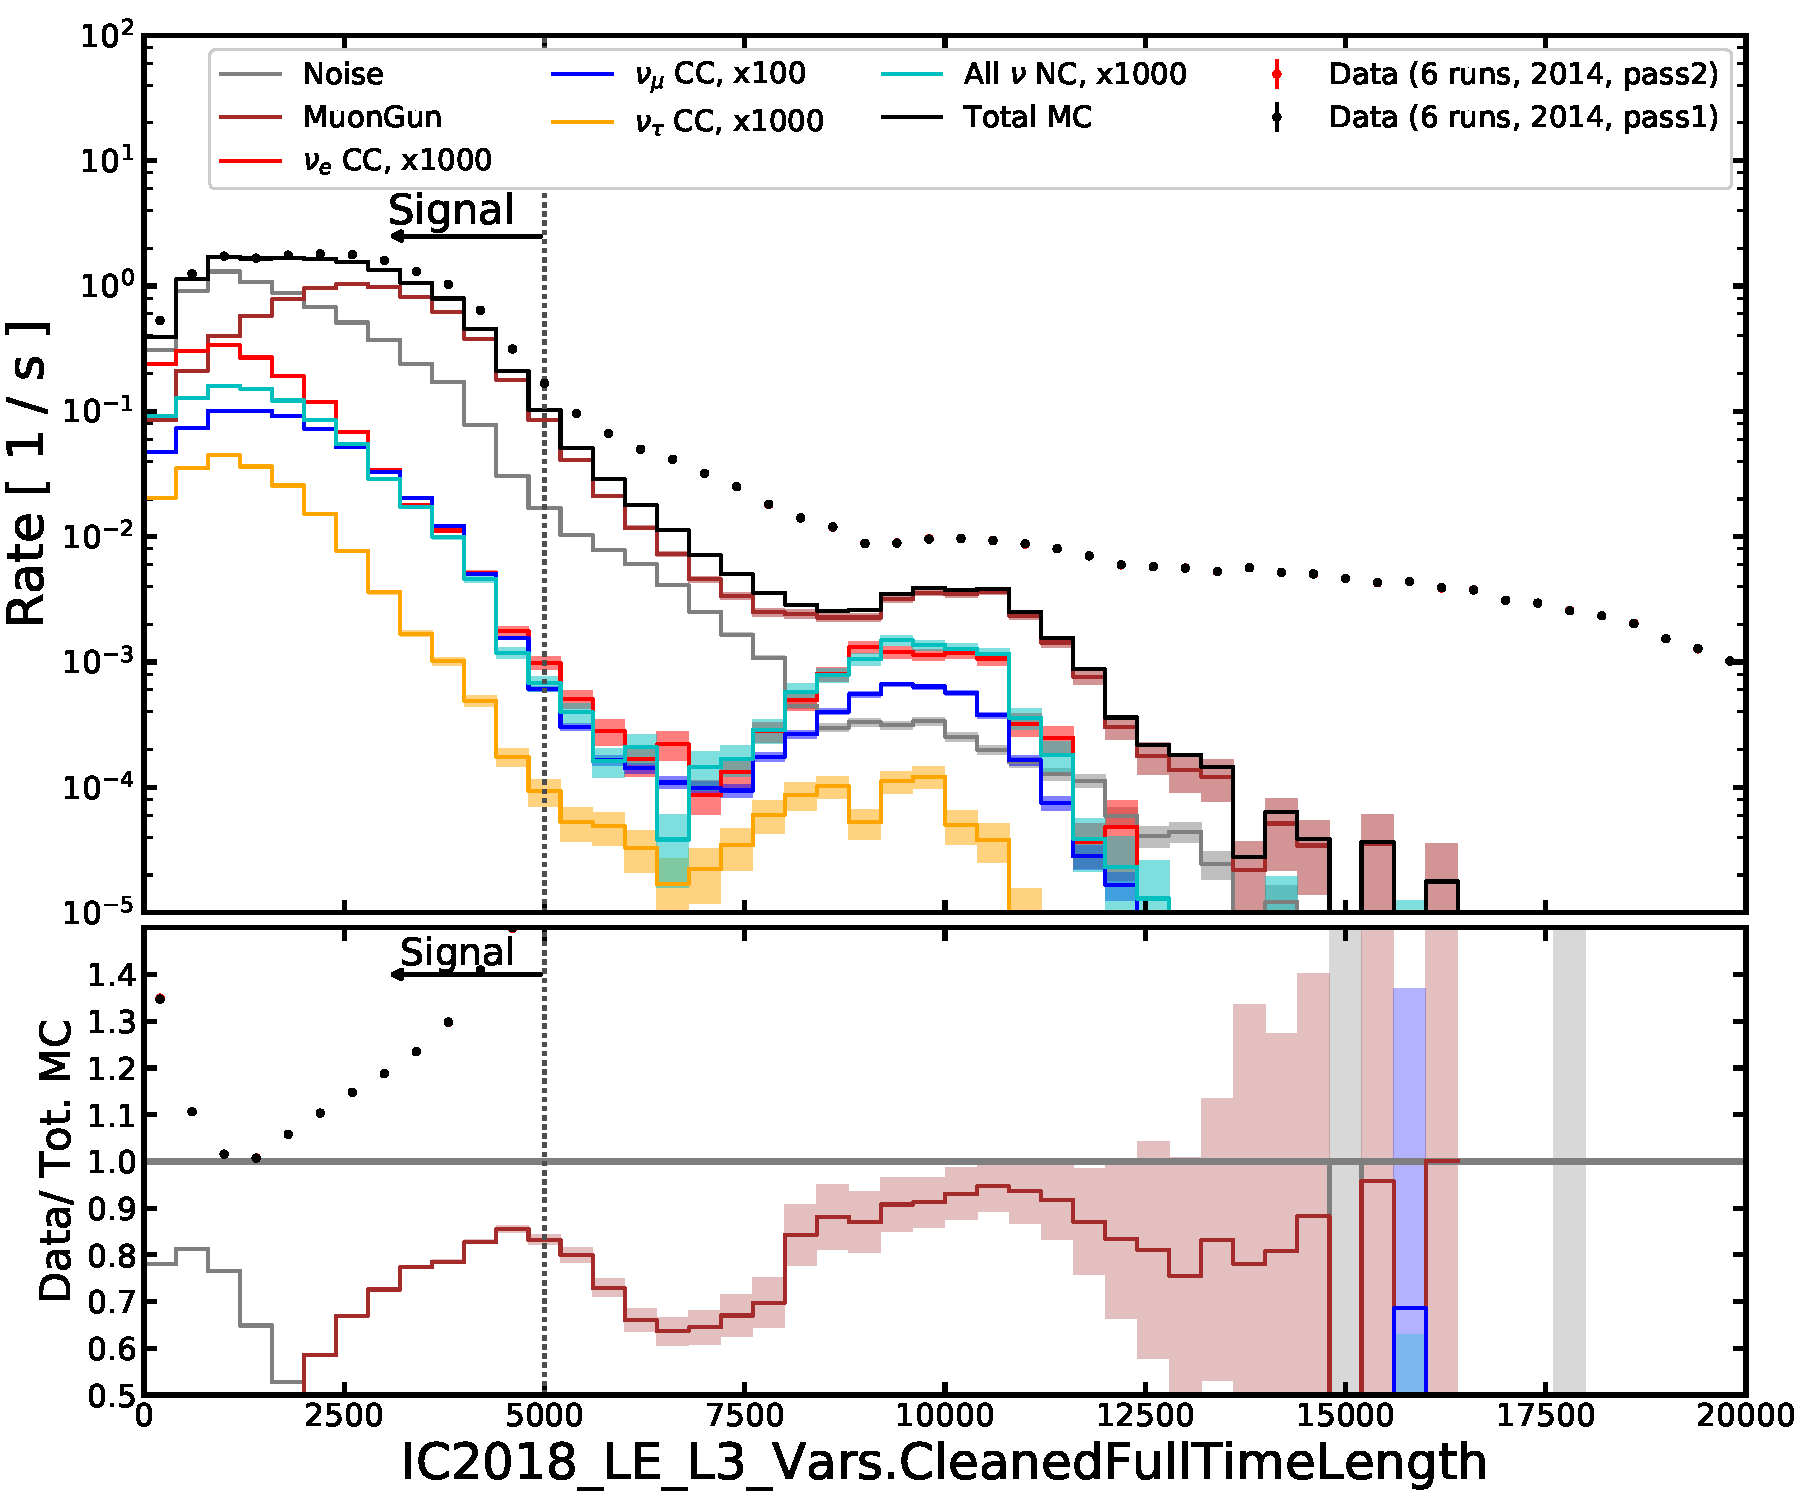
\includegraphics[width=7 cm]{figures/icecube/selection/IC2018_LE_L3_Vars_CleanedFullTimeLength.pdf}
    \caption{Distribution of one of the variables used in the L3 offline filter, the time between the last hit and the first hit after noise cleaning. Histograms show the distributions in simulated data separated by particle and interaction type, data points with error bars show the distribution of real data. The bottom panel shows the ratio between data and simulation. Events falling on the "signal" side of the histogram are passed to the next filter level.}
    \label{fig:l3-var-cleaned-full-time-length}
\end{figure}

\subsubsection{Level 4}
In the next level, L4, more advanced selections based on the output of Boosted Decision Trees (BDTs) are applied, with a separately trained BDT for noise and muon rejection, respectively. The output of each BDT is a probability score between zero (background-like) and one (signal-like).  The inputs into the BDT aimed at noise rejection consist of hit counts in cleaned hit series and variables that characterize the geometric and temporal spread of the observed hits, such as the full width half maximum (FWHM) of the hit times. The BDT is trained using simulated pure noise and neutrino events. Events are passing the L4 noise cut if the BDT score is above 0.7, which reduces the number of pure noise events by two orders of magnitude from 36.6~mHz to approximately 0.3~mHz. The BDT that is used to reject atmospheric muons also takes simple variables as its input that consist mostly of different veto hit counts and variables that characterize the distribution of z-coordinates of the observed hits as well as their radial distance with respect to the center of the DeepCore fiducial volume. In contrast to the noise BDT, however, the muon BDT is trained using real data and simulated neutrino events, with the goal of rejecting data events. This is possible because the data sample consists to 99\% of atmospheric muons at this stage of the event selection. Events are passing the L4 muon cut if the output score from the muon BDT is above 0.65, removing 94\% of all muon events while keeping 87\% of all neutrinos. The distributions of the output scores of both BDTs are shown in figure~\ref{fig:l4-bdt-output}.
\begin{figure*}
    \centering
    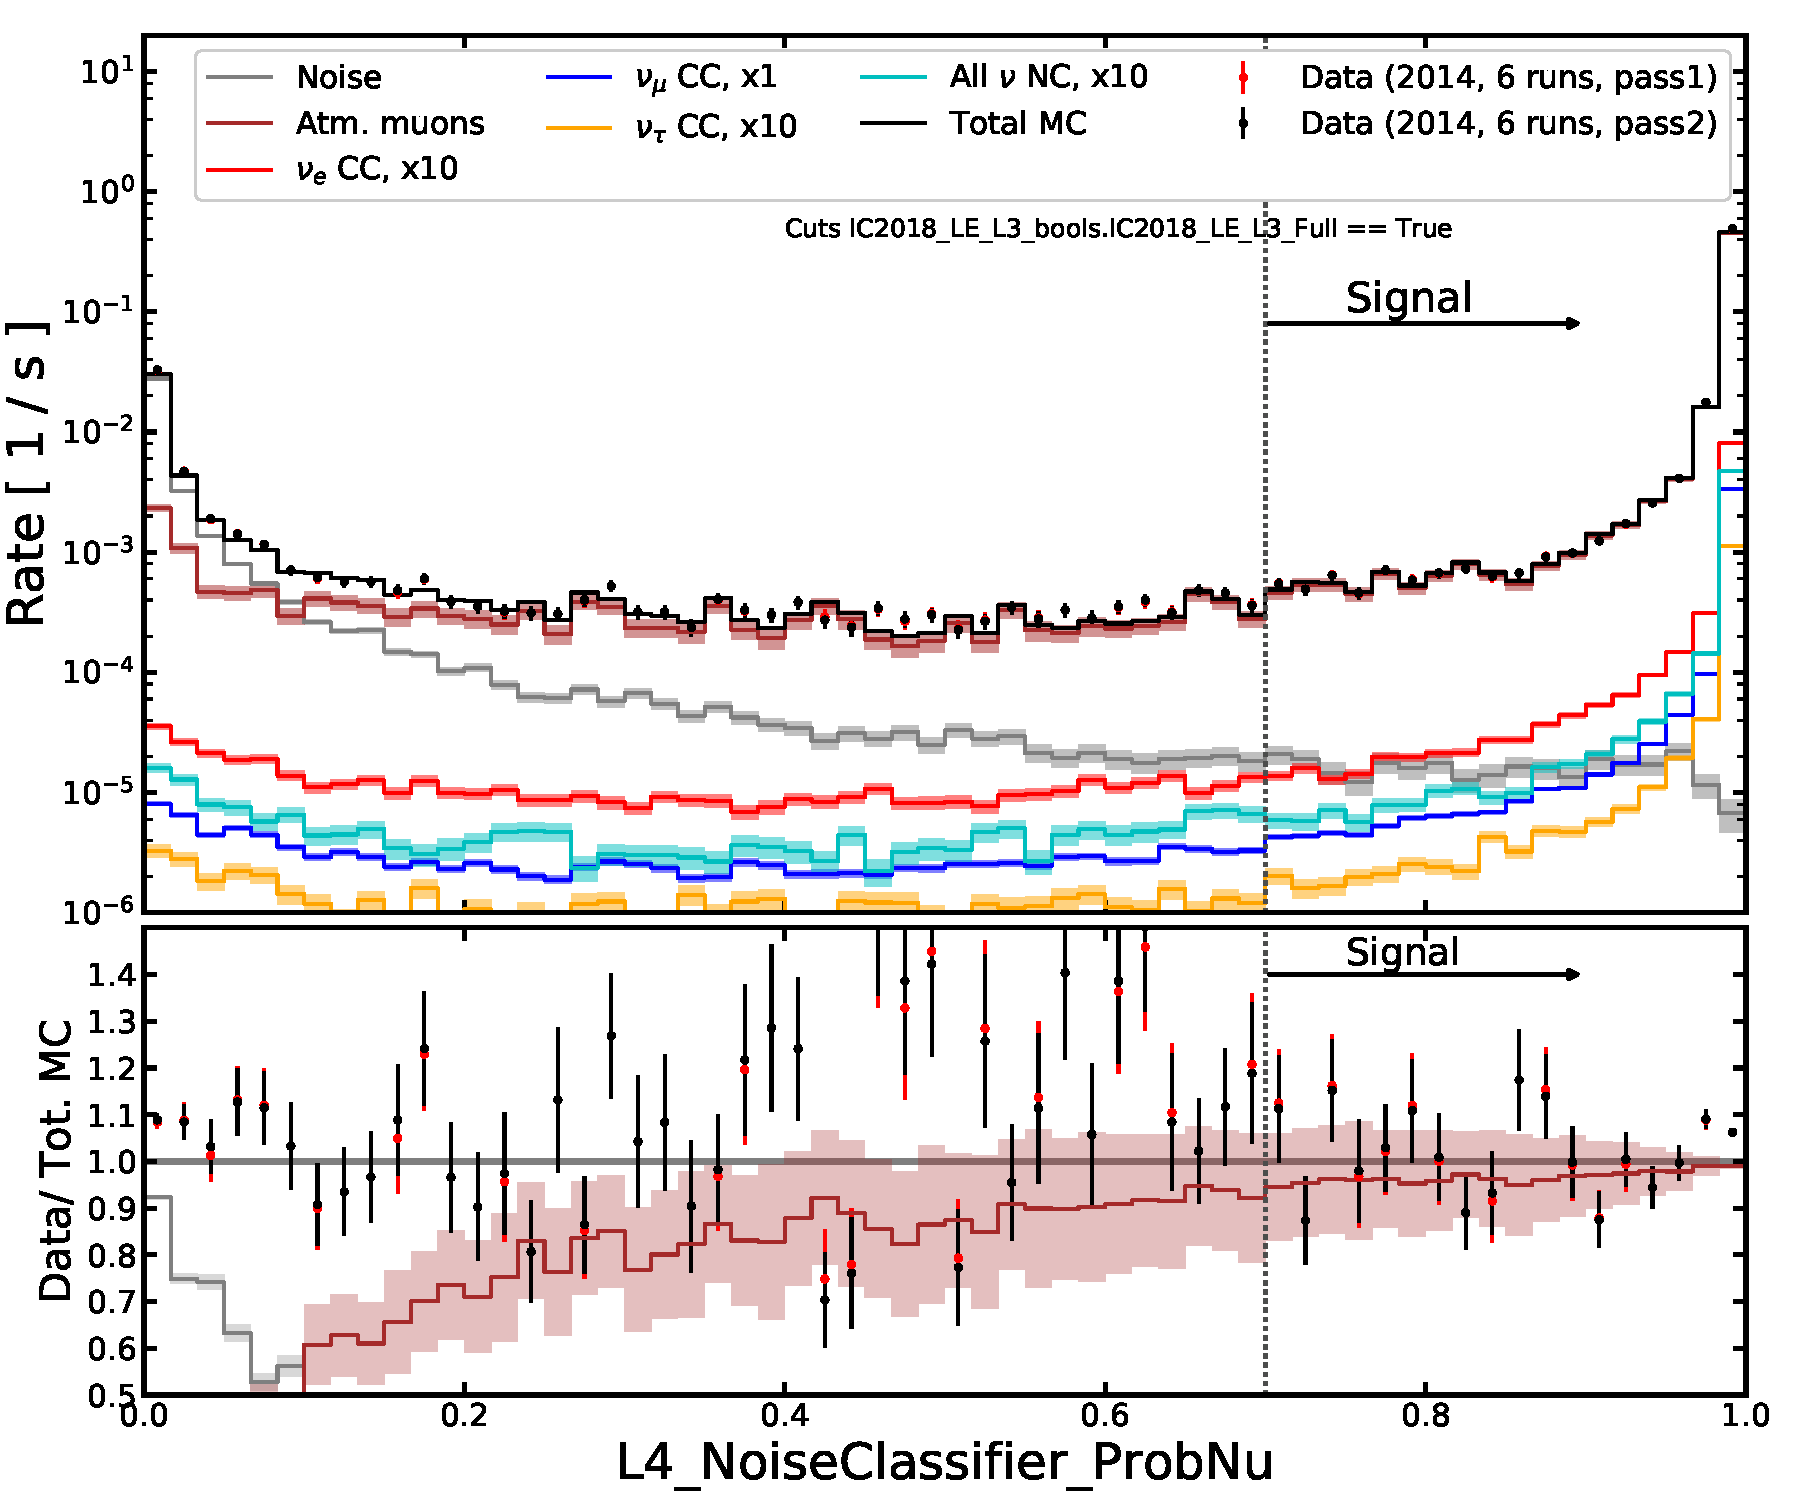
\includegraphics[width=7 cm]{figures/icecube/selection/L4_noiseBDT_L4_NoiseClassifier_ProbNu.pdf}
    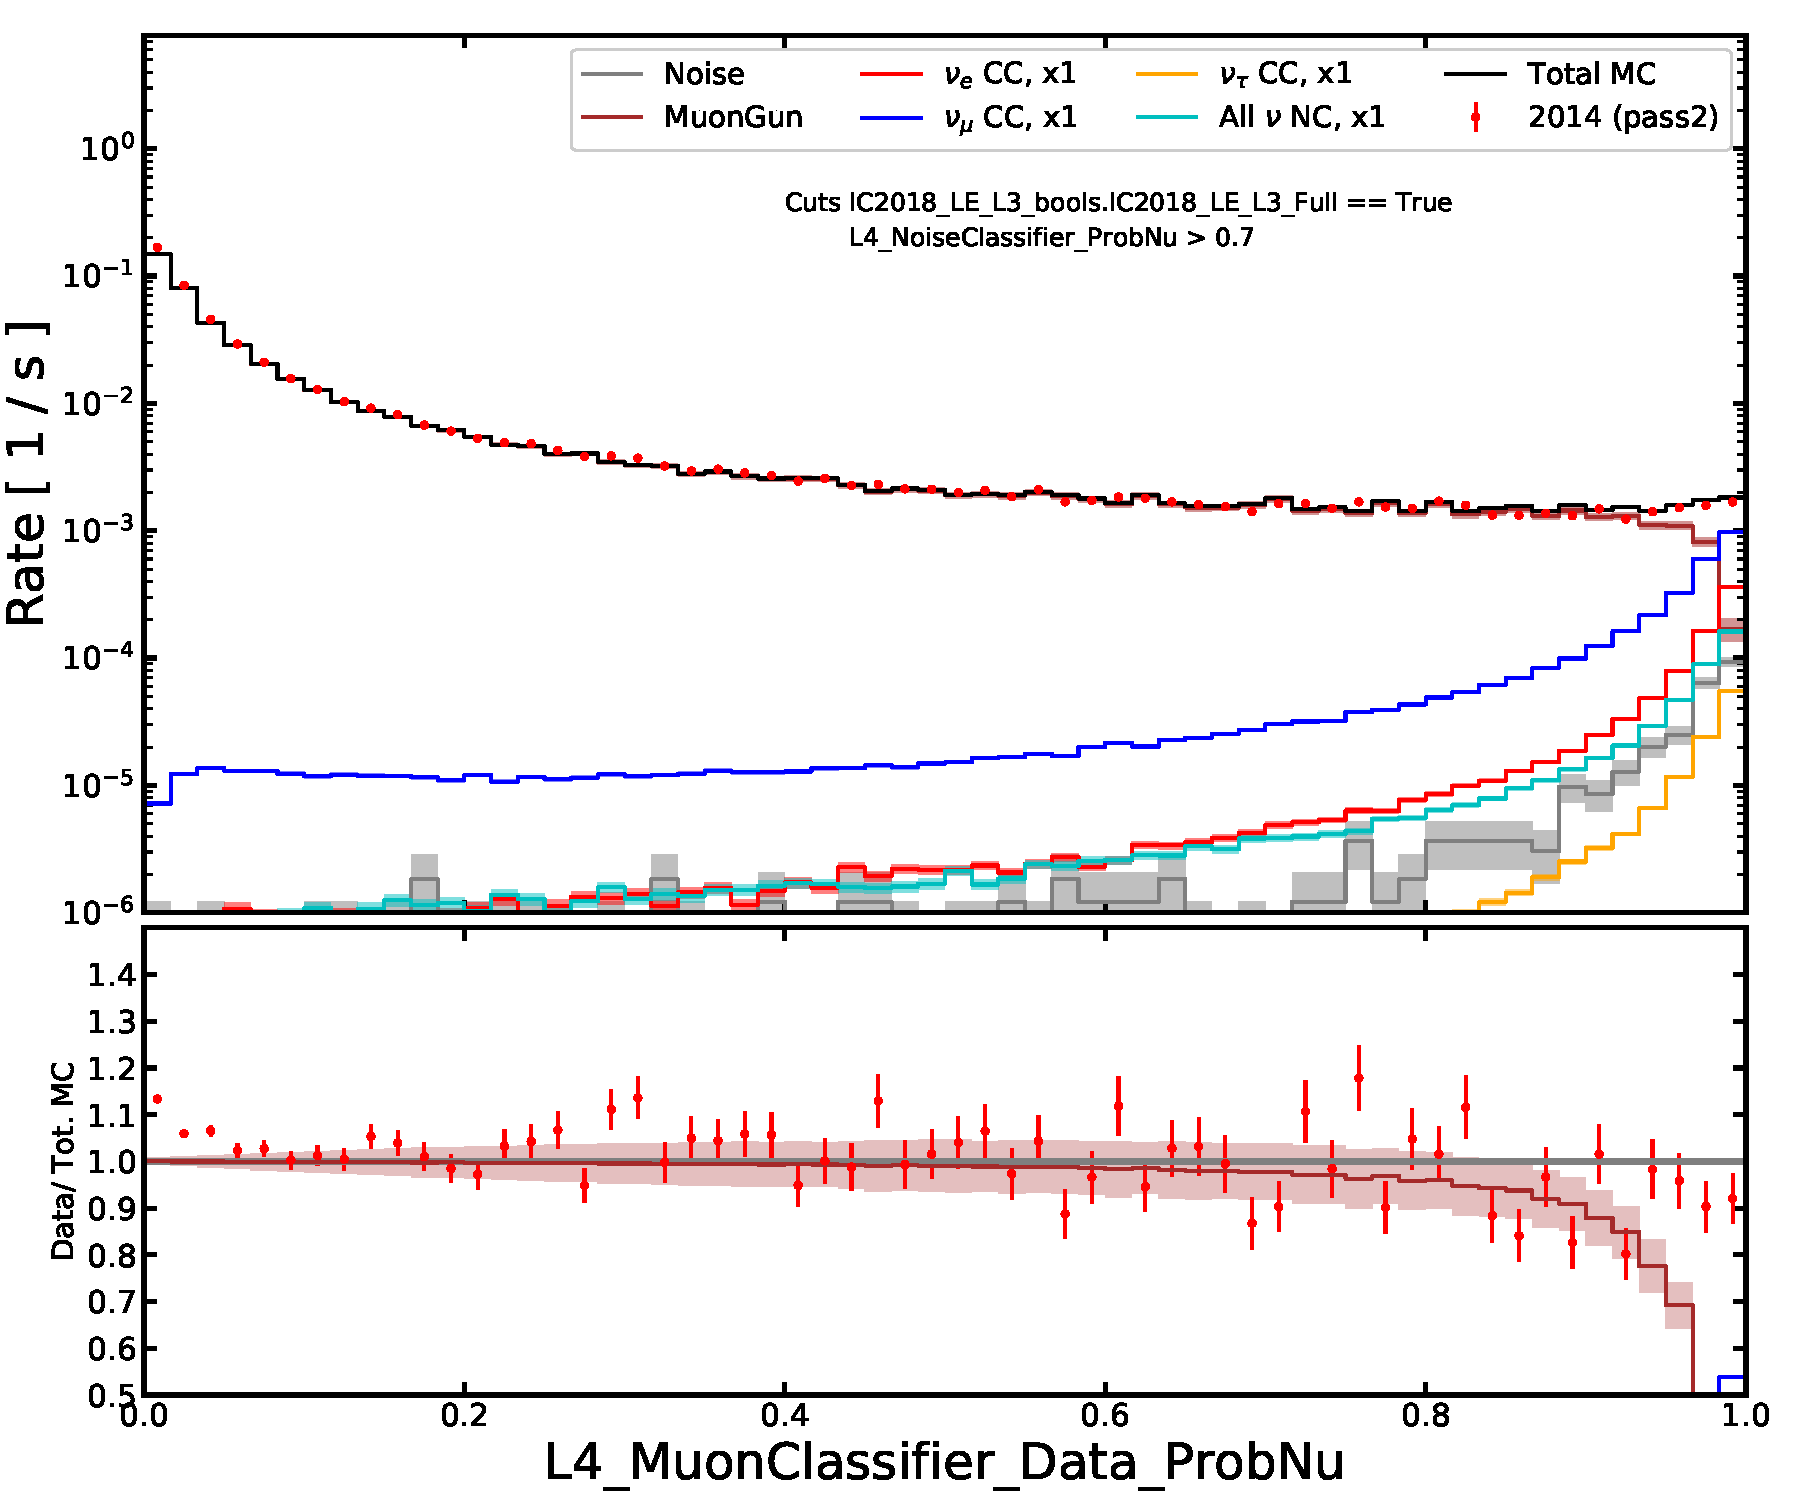
\includegraphics[width=7 cm]{figures/icecube/selection/L4_muon_L4_MuonClassifier_Data_ProbNu.pdf}
    \caption{Distribution scores for the noise (left) and muon (right) BDT. The distributions of the muon classifier are shown for events where the score of the noise BDT is greater than 0.7.}
    \label{fig:l4-bdt-output}
\end{figure*}

\subsubsection{Level 5}
The final offline filter level that is applied before the event reconstruction step is L5. This filter searches specifically for hits occurring in un-instrumented \emph{corridors} within the IceCube array through which an atmospheric muon can sneak into the DeepCore volume while evading previous veto cuts. In addition, events with more than seven hits in the outermost strings of the IceCube array or that have a down-going pattern of hits in the uppermost region of the detector are vetoed to remove events containing atmospheric muons entering the detector coincidentally with neutrinos. The distribution for one of the corridor variables and one of the muon rejection variables are shown in figure~\ref{fig:l5-vars}. Table~\ref{tab:l5_summary} shows the rates of each event type expected at each level of the selection up to L5 together with the efficiency of the filter at the final level.
\begin{figure*}
    \centering
    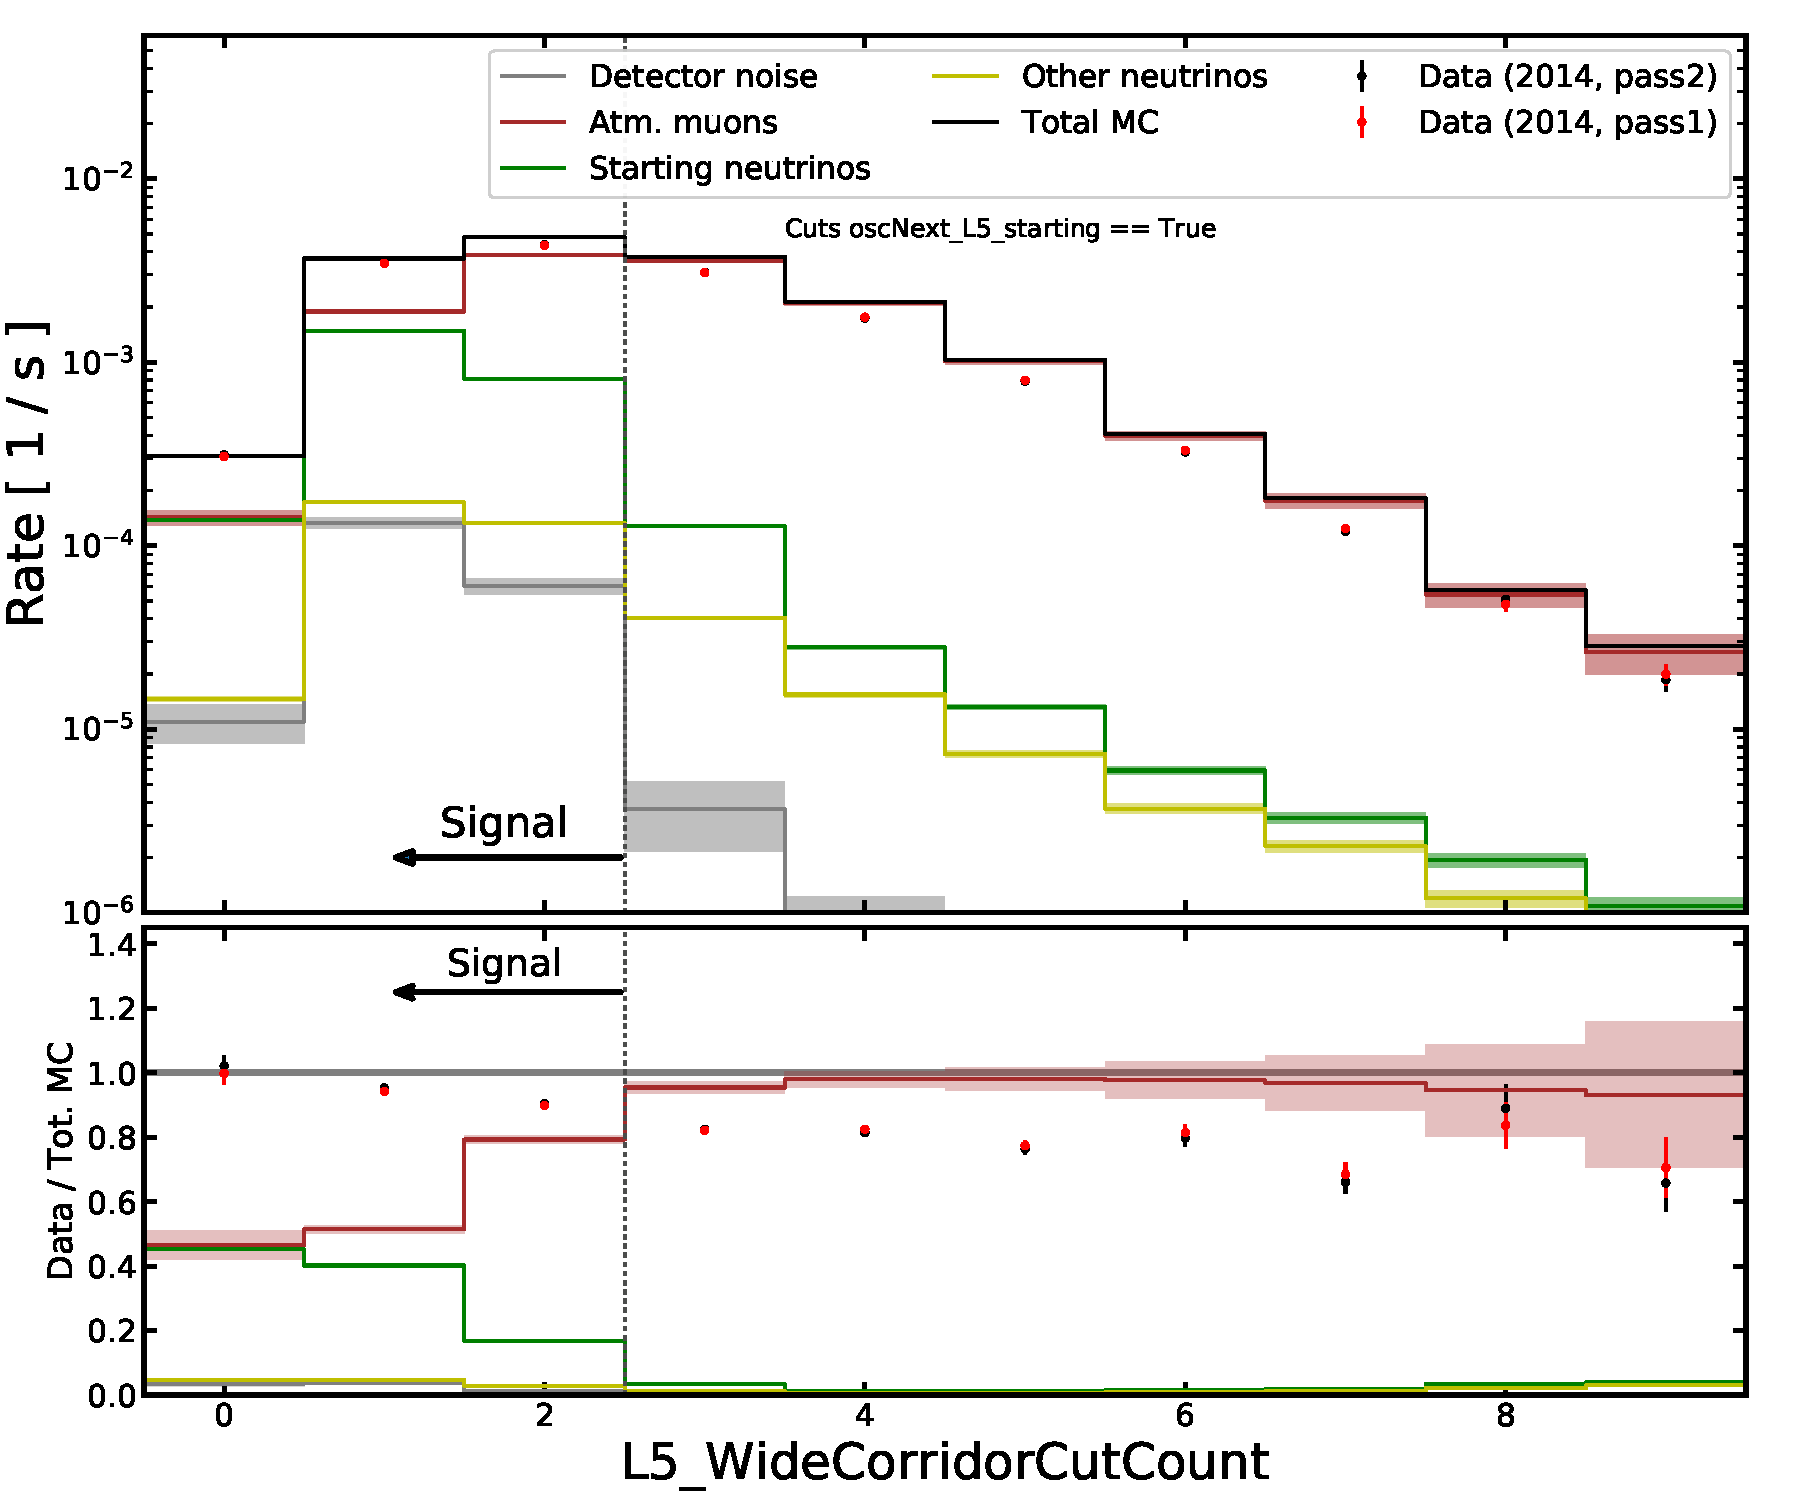
\includegraphics[width=7 cm]{figures/icecube/selection/L5_contained_L5_WideCorridorCutCount.pdf}
    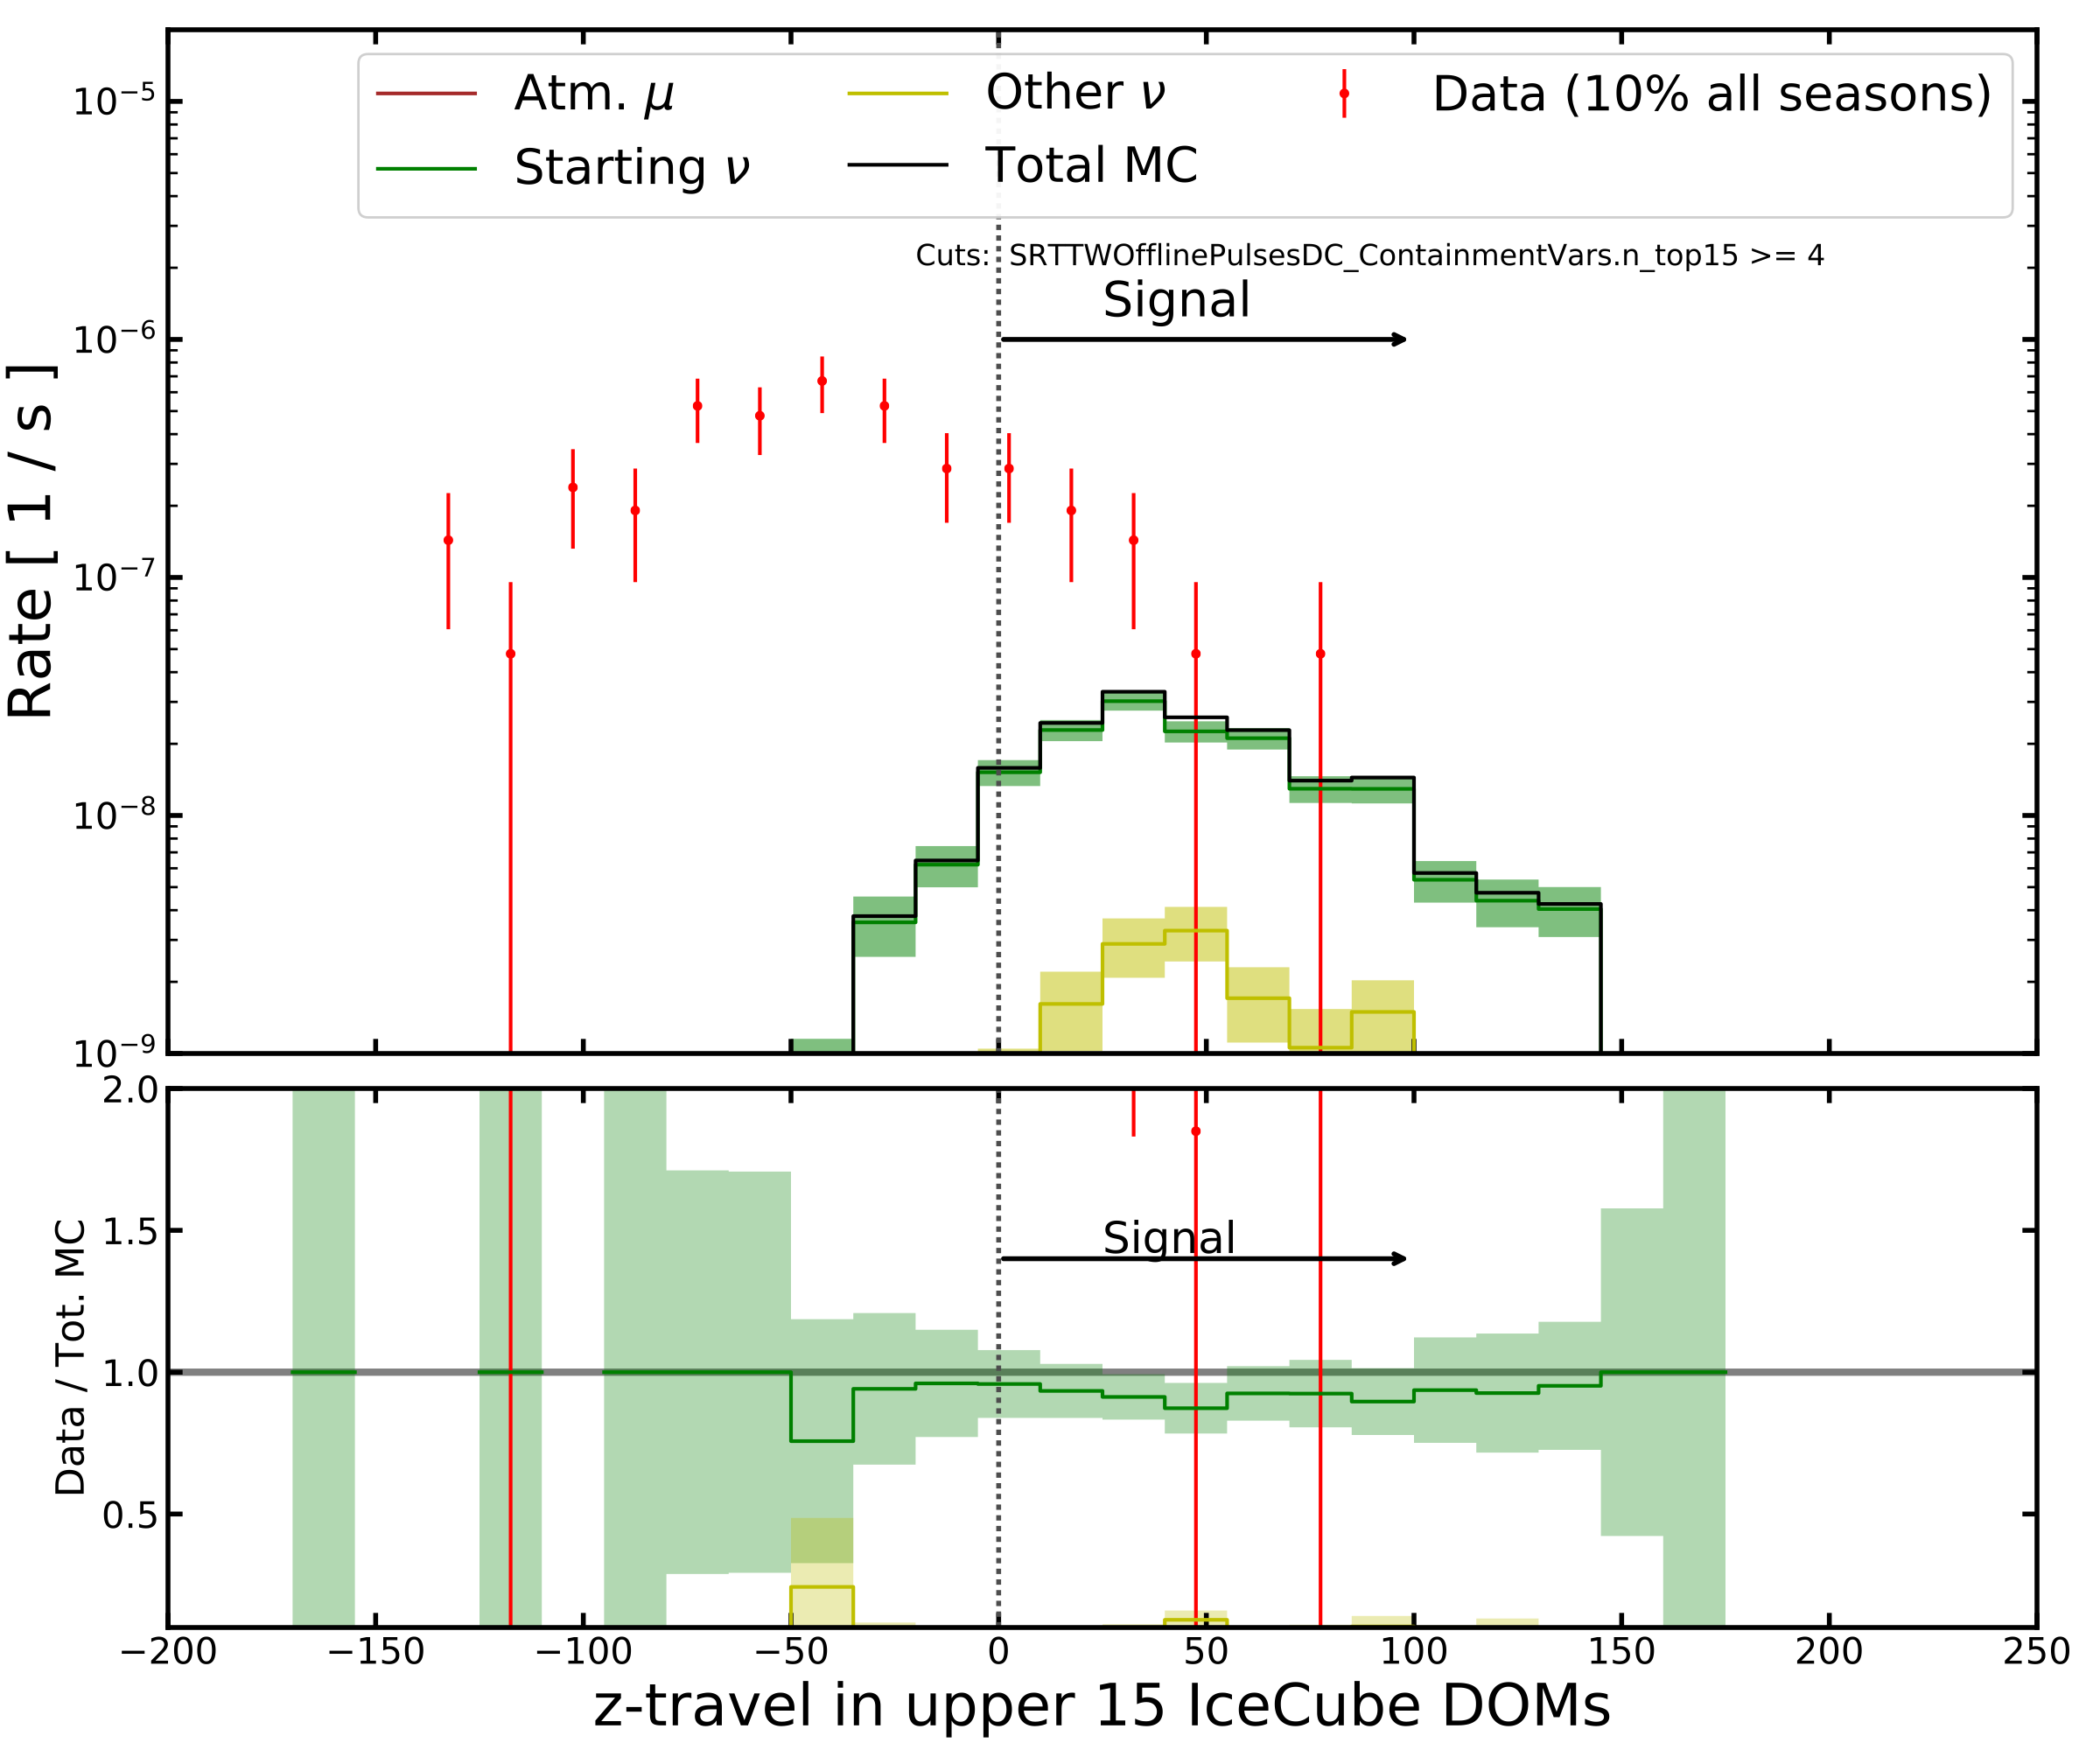
\includegraphics[width=7 cm]{figures/icecube/selection/SRTTWOfflinePulsesDC_ContainmentVars.z_travel_top15.png}
    \caption{Distributions for one of the L5 corridor cut variables (left) and one of the variables used to reject coincident muon events (right). The distribution in the right panel is shown only for events which have at least four hits in the uppermost 15 DOMs combined over all IceCube strings.}
    \label{fig:l5-vars}
\end{figure*}

\begin{table}
\begin{tabular}{lrrrrr}
Event type  & DC filter   & L3   & L4   & L5   & Eff. (\%) \\
\toprule
Atm. $\mu$         & 7273 & 505  & 28.1 & 0.93 & 0.012          \\
Pure noise         & 6621 & 36.6 & 0.28 & 0.07 & 0.001          \\
Atm. $\nu_e$ CC    & 1.61 & 0.95 & 0.84 & 0.48 & 29.8           \\
Atm. $\nu_\mu$ CC  & 6.16 & 3.77 & 3.11 & 1.39 & 22.5           \\
Atm. $\nu_\tau$ CC & 0.19 & 0.13 & 0.12 & 0.07 & 36.8           \\
Atm. $\nu$ NC      & 0.86 & 0.53 & 0.46 & 0.23 & 26.7  \\
\end{tabular}
\caption{Summary of the rates (in mHz) obtained after each level of selection. Neutrinos are weighted to an atmospheric spectrum with oscillations included.}
\label{tab:l5_summary}
\end{table}

\subsection{Event Reconstruction}
\label{sec:event-reconstruction}

After the L5 selection, the rate of muons is reduced enough such that the majority of the total sample is expected to consist of atmospheric neutrinos, and it is at this point that the event reconstruction and signature classification is run. For the measurement presented in this thesis, three reconstructed quantities are required: The zenith angle, the energy, and a proxy score that determines the flavor of a neutrino. As described in section \ref{sec:particle-signatures}, all neutrino events in DeepCore can be effectively approximated as either a cascade ($\nu_e$ CC events, all NC events, and 83\% of $\nu_\tau$ CC events) or a combination of a cascade at the neutrino interaction point with an out-going muon track ($\nu_\mu$ CC events and 17\% of $\nu_\tau$ CC events). The zenith angle can be most accurately reconstructed for track-like events due to their elongated, highly directional signature. For cascades, the reconstruction of the direction is more difficult because of their most compact and diffuse light distribution. The energy of a neutrino event is reconstructed by comparing the expected light output of a combined track and cascade hypothesis to the observed hits. Finally, the flavor proxy is calculated using variables that characterize the elongation of the observed hit signature  and the goodness-of-fit of a combined track and cascade hypothesis compared to that of a cascade-only hypothesis. The resulting score allows the separation of muon neutrino interactions from other interactions, which is ideally suitable to observe the muon neutrino disappearance oscillation channel.

\subsubsection{Zenith angle reconstruction}
The zenith angle is reconstructed using the Single-string Antares-inspired Analysis (\textsc{santa})\sidecite{Garza2014Measurement}. It is an older algorithm aimed at reconstructing the direction of muon tracks that has been originally developed for use in the ANTARES neutrino telescope~\sidecite{Aguilar:2011zz}. It has since been refurbished and improved in IceCube as described in detail in~\sidecite{lowen-reco-paper}.

The reconstructed pulse series in every DOM is summarized by the time of the first pulse and the sum of charges of all pulses. This time and charge is the only information used by the reconstruction and is referred to as a \emph{hit} in the following. The first step of the reconstruction algorithm is a cleaning routine that removes hits produced
by photons that have been scattered many times as they traveled
through the ice, leaving only hits from photons that have travelled in approximately straight lines based on the time difference between hits on the same string.
%The algorithm is a simplification from an earlier implementation described in \cite{Garza2014Measurement}.
It calculates the signal speed between hits on the same string, and removes a hit if this velocity is below the speed of light in ice. This is a simplification from the algorithm described in \cite{Garza2014Measurement}, where the effective signal velocity was updated during the selection process. The selection is run separately for each string, and if fewer than three hits remain on a string, all hits on the string are discarded. In total, it is necessary that at least five hits remain in an event in order to run the directional reconstruction. If only hits on one string remain after the selection, the event is referred to as a \emph{single-string} event, otherwise it is a \emph{multi-string} event. The reconstruction is generally more accurate for multi-string events, because the spacing between strings provides a long lever arm to constrain the direction of a track. In addition, the azimuth angle of the track can only be reconstructed for \emph{multi-string} events due to the rotationl symmetry of a single string.

\begin{figure*}
    \centering
    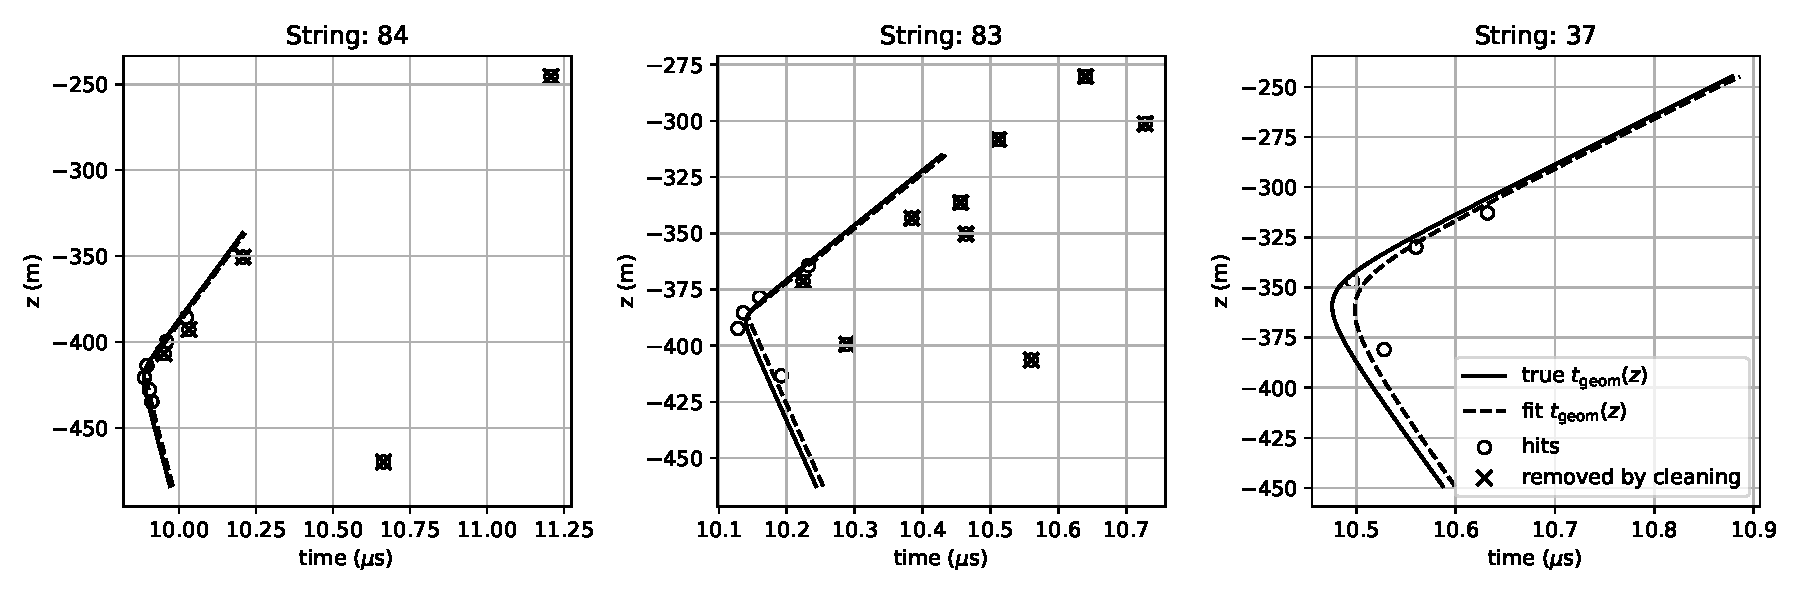
\includegraphics[width=\linewidth]{figures/icecube/reconstruction/santa/multi_string_example_with_cleaning_id_12607962.pdf}
    \caption{Example of a \numucc event reconstructed with \textsc{santa} with hits on several strings. Strings 84, 83 and 37 are spaced $\sim80\,\mathrm{m}$ apart from each other and form a highly obtuse triangle.}
    \label{fig:santa-multi-string-example}
\end{figure*}

The directional reconstruction itself is a regression minimizing a modified $\chi^2$ loss function with respect to the observed and predicted observation time with an additional regularization term involving the observed charge. Given a set of parameters characterizing the track, $\vec{\theta}$, the loss function is defined as
\begin{equation}
L(\vec{\theta})=\sum_{i=1}^{N}\phi(r^2_i(\vec{\theta}))
+
\frac{1}{\bar{q}}\sum_{i=1}^{N}\tilde{q}_i \frac{d_{\gamma,i}}{d_0}\,.\label{eq:chi-square-mod-loss}
\end{equation}
where $\bar{q}$ is the average of $\tilde{q}_i$, and $r^2_i$ is the chi-square residual for each observed hit, $i$, between the observed time, $t_{\mathrm{obs}, i}$ and the geometric arrival time, $t_{\mathrm{geom},i}(\vec{\theta})$,

\begin{equation}
r_{i}^{2}(\vec{\theta})=\left(\frac{t_{\mathrm{geom},i}(\vec{\theta})-t_{\mathrm{obs},i}}{\sigma_{t}}\right)^{2}\,.
\end{equation}

The residual is wrapped in a \emph{robust loss function}, $\phi(r_{i}^{2})=\log\left(1+r_{i}^{2}/C^2\right)C^2$, that grows much more slowly than $r_{i}^{2}$ for values of $r_i$ larger than $C$ while behaving very similar to $r_i^2$ for values of $r_i$ smaller than $C$. Effectively, this robust loss reduces the influence of hits that pass the hit selection procedure despite having undergone a significant amount of scattering. The uncertainty on the pulse time measurement is approximately $\sigma_{t}=3\,\mathrm{ns}$, corresponding to the readout rate of the modules~\cite{icecube_daq}.
The expected arrival time for unscattered Cherenkov photons is calculated geometrically under the assumption of an infinitely long track characterized by a normalized direction vector $\vec{u}=(u_{x},u_{y},u_{z})$,
an anchor point $\vec{q}=(q_{x},q_{y},q_{z})$ and a time $t_{0}$
at which the particle passes through $\vec{q}$. The
velocity is fixed to the vacuum speed of light, $c$. Since the reconstruction ignores DOMs that have not recorded any pulses, the fact that the true track length is finite only makes a negligible  difference.
Without scattering, all Cherenkov photons lie on a cone with an opening
angle $\theta_{c}$ (see Fig.~\ref{fig:Detailed-track-geometry})
\begin{figure}[h]
\begin{centering}
\tikzsetnextfilename{track_geometry_santa}%
\begin{tikzpicture}[scale=1,>=stealth]
	\path[name path=track] (0,3) -- (9,3);
	\node[shape=star,
	      star point height=1cm,
	      star point ratio=0.5,
	      draw, fill=black,
	      label=below:$\vec{p}(t_{\mathrm{em}})$] (emission) at (1,3) {};
	\draw[->, decorate,
	decoration={snake,amplitude=.4mm,segment length=2mm,post length=1mm}]
		(emission.center)
		-- node[sloped, above] {$d_{\gamma}$} +(40:4)
		node[label=above:DOM at $\vec{r}$] (dompos) {};
	\path[name path=cone] (dompos.center) -- +(-50:4);
	\draw[name intersections={of=track and cone, by=tip}]
		(dompos.center) -- node[sloped, above] {Cherenkov light cone} (tip)
		node[label=below:$\vec{p}(t_{\mathrm{geom}})$] (muonpos) {};
	\draw[fill=black, opacity=0.5] (dompos.center) circle (5pt);
	\draw[color=black, ->, style=very thick] (0,3) node[anchor=north]{muon} -- (muonpos.center);
	\draw (emission.center) +(1,0) node[anchor=south east]{$\theta_c$}  arc (0:40:1);
	\path (emission.center)
		-- node[shape=circle,
			fill=black,
			label=below:$\vec{q}$] (vertex) {}
		(tip);
	\draw[->] (vertex.center) -- node[sloped, below] {$\vec{r}-\vec{q}$} (dompos.center);
	%\draw (vertex.center) +(-1,0) arc (180:140:1);
	%\path (vertex.center) -- +(160:0.6) node {$\theta$};
	\draw[->] (vertex.center) ++(0.2, 0.2) -- node[above] {$\vec{u}$} +(1,0);
\end{tikzpicture}\par
\end{centering}
\caption{\label{fig:Detailed-track-geometry}Detailed geometry of a light cone
created by a track. $\vec{q}$ is the position of the anchor point
and $\vec{r}$ is the position of the optical module. $\vec{p}(t_{\mathrm{em}})$
and $\vec{p}(t_{\mathrm{geom}})$ are the positions of the muon at
the time the photon is emitted and when it is geometrically expected
to arrive, respectively.}
\end{figure}
whose tip is at the position of the particle at the time $\vec{p}(t)$. The opening angle satisfies $\cos(\theta_c)=1/n_{\mathrm{ph}}$, where $n_{\mathrm{ph}}$ is the phase index of refraction of the ice.
Assuming that a photon has travelled in a straight line at the group velocity in ice, the geometric arrival time, $t_{\mathrm{geom}}$, for a DOM at position $\vec{r}$ is

\begin{equation}
t_{\mathrm{geom}}=t_{0}+\frac{1}{c}\left(\left(\vec{r}-\vec{q}\right)\cdot\vec{u}+\frac{d_{\gamma}}{n_{\mathrm{ph}}}\left(n_{\mathrm{ph}}n_{\mathrm{gr}}-1\right)\right)\label{eq:t_geom-MS-track}
\end{equation}
where the distance traveled by the photon $d_\gamma$ is
\begin{equation}
d_{\gamma}=n_{\mathrm{ph}}\sqrt{\frac{1}{n_{\mathrm{ph}}^{2}-1}\left(\vec{u}\times\left(\vec{r}-\vec{q}\right)\right)^{2}}\,.\label{eq:photon-distance-3d}
\end{equation}

\begin{figure}
    \centering
    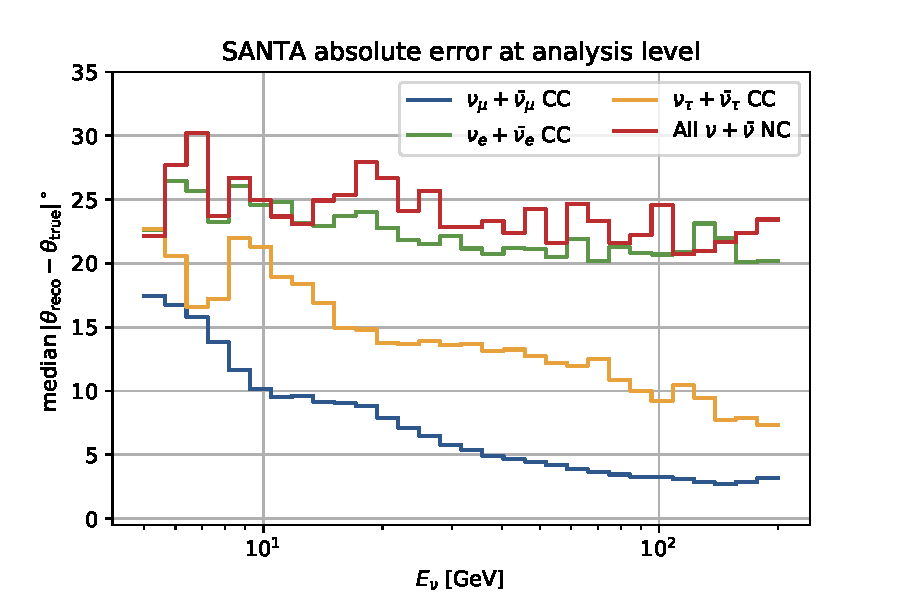
\includegraphics[width=0.7\linewidth]{figures/icecube/reconstruction/santa/santa_absolute_error_final.pdf}
    \caption{Median error on the reconstructed zenith angle at the final level of the sample selection as a function of neutrino energy.}
    \label{fig:santa-resolution}
\end{figure}

The group and phase indices of refraction depend on the wavelength, but for this reconstruction the value for a wavelength of $\lambda=400\;\mathrm{nm}$
\footnote{$400\;\mathrm{nm}$ is near the wavelength of the highest acceptance of the optical modules.\cite{icecube_detector_17}} is used, where $n_{\mathrm{gr}}=1.356$ and $n_{\mathrm{ph}}=1.319$~from~\sidecite{PRICE200197}. An example of a simulated event reconstructed with \textsc{santa} is shown in figure~\ref{fig:santa-multi-string-example}. The solid and dashed lines show the geometric arrival time calculated according to equation~\ref{eq:t_geom-MS-track} using reconstructed and true track parameters, respectively. The circles indicate hits in DOMs, and those hits that have been removed by the hit cleaning procedure are crossed out. The median error on the zenith angle reconstructed using \textsc{SANTA} is shown in figure~\ref{fig:santa-resolution}, split by neutrino interaction type. As expected, the error is smallest for $\nu_\mu$-CC interactions, since those produce track signatures that most closely resemble the infinite track hypothesis underlying the \textsc{SANTA} reconstruction algorithm. The worst resolution is achieved for interactions that only produce electronic or hadronic showers, since they produce cascade signatures hardly resembling the infinite track assumption. It is also apparent that the median resolution for $\nu_\tau$-CC events lies between that of $\nu_\mu$-CC events and pure cascade events. This is readily explained by the fact that 17\% of these interactions also produce a muon in their final state.

\subsubsection{Energy reconstruction}

The energy reconstruction runs as a separate step after the zenith angle reconstruction. In contrast to \textsc{SANTA}, the energy reconstruction fits a combined hypothesis consisting of a cascade and a track of finite length originating at the same point of the cascade. Both the cascade and the track are constrained to move only along the infinite track that has been fit in the zenith reconstruction. This means that the model fit in the energy reconstruction is fully characterized by the shift of the vertex along the infinite track, the length of the finite track (which is linearly related to the track energy), and the energy of the cascade. Given these parameters, the expected light yield for all DOMs is calculated using so-called \emph{photonics tables}. The tables consist of B-spline coefficients that have been fit to simulated photon propagation for cascades and 3~m long tracks segments at different depths and directions inside the IceCube array to give a (time-dependent) expectation value for the photon count at arbitrary positions inside the detector. The expectation of an arbitrarily long track is calculated by chaining the 3~m segments together that fully cover the desired track length, and scaling the amplitude of the last segment by the remainder of the division of the desired length by the length of the segments. Given these expectation values as a function of event parameters, $\lambda_i(\theta)$, for every DOM, $i$, a simple Poisson ''hit vs. no-hit'' log-likelihood is calculated as
\begin{equation}
    \log(\mathcal{L}) = \sum_{i\in\mathrm{DOMs\;without\;hits}} e^{-\lambda_i(\theta)} + \sum_{i\in\mathrm{DOMs\;with\;hits}} (1 - e^{-\lambda_i(\theta)})\;.
    \label{eq:leera-llh}
\end{equation}
This likelihood is maximized under the hypothesis that the shift, track length, and cascade energy are all free parameters, and under the alternative hypothesis where the track length is fixed to zero, the latter of which corresponds to a cascade-only hypothesis. The difference between these two log-likelihoods provides a measure of the degree to which the ''cascade + track'' hypothesis fits the observed data better than the ''track-only'' hypothesis. It is one of the inputs that are used in a BDT to calculate an over-all score of how track-like an observed event signature is. The median relative error on the reconstructed total energy (i.e. the sum of the track energy and cascade energy) is shown in figure~\ref{fig:leera-resolution}. As with the zenith angle reconstruction, the relative error is smallest for \numucc-events. This is expected, since these events fit the hypothesis of an initial cascade combined with a finite track the best. The second-best resolution is achieved for $\nu_{e,\mathrm{CC}}$-events, while it is poorest for $\nu_{\tau,\mathrm{CC}}$ and neutral-current events. This is explained by the fact that the expected light yield that is put into equation~\ref{eq:leera-llh} is based on the assumption that all particles that are produced in the interaction are visible to the detector. While this assumption is a good approximation for $\nu_{e,\mathrm{CC}}$-events, it does not hold for hadronic cascades that contain some neutral components as discussed in chapter~\ref{sec:had-showers}. The true energy of the primary particles that produce hadronic cascades is therefore systematically under-estimated and has a larger uncertainty. This additional uncertainty is fundamentally irreducible, because it is not possible to distinguish the signatures of hadronic and electromagnetic showers.

\begin{figure}
    \centering
    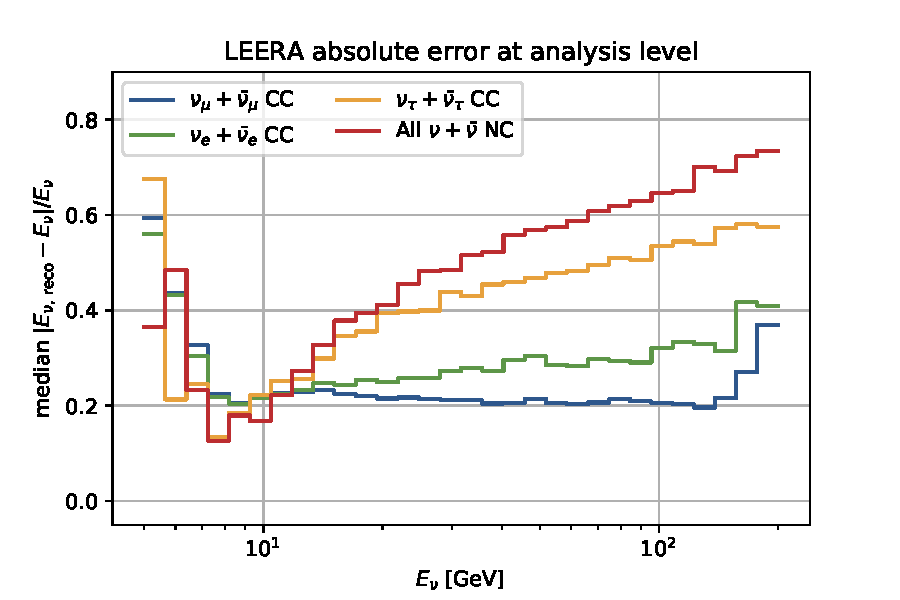
\includegraphics[width=0.7\linewidth]{figures/icecube/reconstruction/leera/leera_absolute_error_final.pdf}
    \caption{Median fractional error on the reconstructed energy at the final level of the sample selection as a function of neutrino energy.}
    \label{fig:leera-resolution}
\end{figure}

\subsection{Signature Classification}

In addition to the energy and zenith angle, the measurement presented in this thesis requires a svore separating track-like \numucc-events from other types of interactions. 